
\section{Tool}
\label{sec:experiments}

In this section, we discuss intuition behind combining HDD with statement deletion mutation to develop \mytool\  such that it fits into adaptation workflow, modified HDD algorithm, architecture, implementation and usage of the tool in detail.       

\subsection{coverage and dead code removal}
It is important to note that if the program parts that can be reduced only contains non covered entities, just computing coverage and removing non covered entities will do the job. But even if entities are covered, but does not contribute to the correctness of program as defined by test suite, they qualify as reduction candidates. Though \mytool\ can be optimized by allowing non covered entities to be reduced first, something we are planning to do in future. To provide an example, consider following code that was removed as part of our reduction from URLValidator class.

\begin{lstlisting}[caption={URLValidator reduced code}]
if (!isValidAuthority(authority)) {
	return false;
}
\end{lstlisting}

The code was reduced when we relaxed specifications by randomly turning off 2 tests. The code was reduced though it was \emph{covered 42018 times during execution}. 

%At any point in the reduction step, we are essentially creating a statement deletion mutant or a combination of multiple statement  though with the purpose of creating a useful version of the program instead of injecting a fault. We start the process from leaf nodes, if we find a useful SDL mutant, we keep it and use it for rest of the process until local minimal is reached.%  


\subsection{1-minimal program}
\label{sec:opensource}

Original delta debugging work defines different notions of minimality for reduction in detail \cite{ddOriginal}. For our further discussion, we define 1-minimal program or 1-minimal mutant as follows. It is important to note that this is local minimal as DD or HDD are greedy and our algorithm is also greedy \cite{ddOriginal, hddOriginal}. Given a program P and a  test suite T, we define 1-minimal (local) program P' of P is the reduced version of P such that all tests continue to pass and the program cannot be reduced further. For component level adaptations, the idea of 1-minimality is applied at component level. The intention of hddRASS is to output the 1-minimal program for a given program given a test suite such that all tests continue to pass. 

\subsection{Statement Deletion mutation - SDL}
\label{sec:sdl}

If resource adaptation is triggered because of resource constraint violation and if a reduced program/component is generated, as the reduced program is still a useful artifact that will continue to function as it is mostly, we hypothesize that small local changes are applied to the program. The newly created program is a perturbation of the original program and mutation captures perturbations well. In traditional mutation testing, purpose of the mutant is to act as an artificial bug while in our case mutant is a useful perturbed version of original program. Rahul write this statement: Statement Deletion mutation operator was proposed by xyz and during empirical analysis conducted by abc it was found to be very effective and it subsumed other mutation operator significantly. When HDD is traditionally applied on programs, it relies on tree structure of the program like AST, CFG or ECFG etc. For example, picireny relied on ECFG of programs. Its reduction run even deeper then program statements, it even reduces expressions. Our approach does not go beyond SDL because (1) SDL operator was found to be subsuming other mutation operator that are used in expressions (2) As reduced program still needs to be working as mostly correct program, we expect simple removals. (3) Minimally reducing expressions, conditions etc further may be very time consuming and hence runtime adaptations may not converge quickly.

   


\subsection{Intuitive modification to HDD for RASS}
\label{sec:intutive}
Now we describe modifications that we propose to original algorithm and intuition behind the proposals. Later during evaluation we find some evidence for the intuition. We need to put on our \emph{Resource Adaptive Software System developer} hat on to understand this modifications. As the reduced adaptive program is a useful artifact that will be used in place of the original software, we hypothesize that (a) it may not be drastically different then the original program. (b) Any reduction that does not compile is useless.

(1)  Reduction may incur many small local changes to software based on the relaxed specifications. As original HDD setups were designed to quickly converge to reduced input that is significantly \emph{smaller} then original input, they tend to make bigger chops earlier in the process. As changes to RASS are going to be local and smaller, we propose modification to original algorithm. Our algorithm always start with leaf nodes at highest depth level and it chops smallest possible unit at the beginning (statements for our tool). 

(2) Consider any two statement s1 and s2 existing at the same level in AST in the order s1,s2. Our algorithm always delete s2 before s1. Our deletions are always from right to left at same level in AST. (a) This prevents some posibilities of non compilable code and hence costly reverts, use will always be deleted before def. (b) Later read/write will be deleted before earlier read/write. Will this have better chance to keep program correct, for Alex to answer? Reverts will be needed only if any test in test suite failed.    

(3) Consider any two statements s1 and s2 existing at different level in AST such that s1 is at higher level. As our algorithm starts from leaf node and moves upward, s2 will be deleted before s1 ensuring that if def and use are at different levels, use will be deleted before def, again reducing possibility of non compilable code.  



\subsection{Algorithm}
The basic algorithm is described below. It still follows all the standard steps of HDD, though it is modified to fit into adaptation workflow better by taking into consideration modification mentioned in previous section. 

\begin{algorithm}
\caption{Hierarchical Delta Debugging}
\hrulefill
\begin{algorithmic}[1]
\Procedure{hdd}{$inputTree$}
    \State $level\gets\textsc{HigestDepthLevel}(inputTree)$
    \State $nodes\gets\textsc{TagNodes}(inputTree,level)$ 
    \While{nodes are not empty}
	\State $minConfig\gets\textsc{ddmin}(inputTree)$
	\State $\textsc{prune}(inputTree,level,minConfig)$
	\State $level = level - 1$
	\State $nodes\gets\textsc{TagNodes}(inputTree,level)$ 	
	\EndWhile

    \State \textbf{return} $level$ 
\EndProcedure
\end{algorithmic}
\hrulefill
\end{algorithm}
\label{sec:algorithm}


\subsection{Architecture and implementation}
\label{sec:architecture}
\begin{figure}
  \centering
  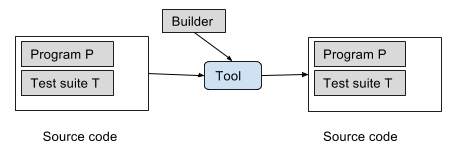
\includegraphics[width=1.0 \columnwidth]{basic_tool_architecture.png}
  \caption{Overview of the tool}
  \captionsetup{justification=centering}
  \label{fig:fig1}
\end{figure}



The basic architecture of the tool from a user's perspective is shown in figure ~\ref{fig:fig1}. For Java-JUnit combo, user just needs to provide the source code that consists of the program and labeled tests for java projects.The only extra information needed is a build command - ant, gradle or maven command for modern day java projects. No separate mechanism is needed to feed DD with pass-fail result by setting up a tester, running it and collecting the results. 

Figure ~\ref{fig:figDetailedToolArch} describes the detailed architecture of the tool. Components in oval gray are input/output, original program P, Test suite T, and builder constitute input and Program P$'$ is output. Components in white rectangle constitute part of the tool. Architecture follows standard HDD/DD procedure of reduction while taking into account the changes proposed in intuitive modification subsection. Program is passed to AST Parser \cite{javaparser}, we used JavaPaser for this. We implemented our own HDD to reflect changes mentioned in intuitive modification subsection. Similarly, we have our own implementation of DD for the reasons mentioned in intuitive modification subsection. Apart from implementation/algorithmic changes that we proposed, the major architectural change consists of how test results are being fed to dd. Tools like picireny and chipperJ require some sort of test script and pre-processing for developers, while testing is built in as part of our tool. 			

\begin{figure*}
  \centering
  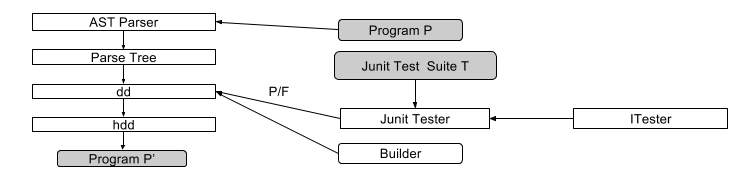
\includegraphics[width=1.8 \columnwidth]{detailed_tool_architecture.png}
  \caption{Architecture of the tool}
  \captionsetup{justification=centering}
  \label{fig:figDetailedToolArch}
\end{figure*}


\subsection{Usage}
Tool takes as its input, a program (or a component if only component needs to be reduced), a test suite or a tester, a build system and produces a \emph{minimally reduced program} such that all test cases continue to pass.  Though right now it works as a stand alone tool with JUnit tests only, the tool is very extendable and flexible to accommodate any other testing technologies. Just like JUnitTester in the ~\ref{fig:figDetailedToolArch}, providing an extra implementation, NUnitTester, will make the tool capable of working with any java projects consisting of NUnit test suite out of the box. Tool can be easily extended to work with other arbitrary tester by implementing a simple interface that consists of only one method. We were able to extend it for TSA system under consideration that has a customized tester written in python by implementing the interface using less then 70 lines of java code. Tool is made available as command line tool with many flexible options giving developers very fine control over how it can be used. Tool can be used at method level, class level, program level or component level giving its user finer control over reduction. 








\subsection{Challenges}
The challenges that we faced are very similar to other reduction tools. 

\begin{enumerate}
\item Non complilable code - Most of other tools discussed in this paper, just revert the code if code is not compilable at any step of reduction. This issue is not present in our implementation by design, we attempt to produce code that compiles only. Though we still compile at the end of each reduction step (just like other tools) in order to make sure that our reductions are at any point of time are compilable indeed. Because of our proactive approach, we are able to avoid reverting, one of the most time consuming step, reverting mostly require writing back java files. 
\item Infinite loops - This problem is just not avoidable as reduction can delete loop control statements. We employ very crude strategy of providing some threshold and giving up if the threshold is hit and returning Fail as result of tests. 
\item Local minimum - As mentioned earlier, nature of ddmin or hdd just produces local minimum and as our tool is built on hdd, our tool also produces local minimum program.
\end{enumerate}




